\documentclass[portrait,b1paper,fontscale=0.410]{baposter}

\usepackage[brazil]{babel}
\usepackage[utf8]{inputenc}
\usepackage{times}
\usepackage{calc}
\usepackage{url}
\usepackage{graphicx}
\usepackage{amsmath}
\usepackage{amssymb}
\usepackage{relsize}
\usepackage{multirow}
\usepackage{booktabs}
\usepackage{graphicx}
\usepackage{multicol}
\usepackage[T1]{fontenc}
\usepackage{ae}

\graphicspath{{fig/}}

% Multicol Settings
\setlength{\columnsep}{0.7em}
\setlength{\columnseprule}{0mm}

% Formating
\newcommand*{\norm}[1]{\mathopen\| #1 \mathclose\|}
\newcommand*{\abs}[1]{\mathopen| #1 \mathclose|}
\newcommand*{\dd}{\partial}
\newcommand*{\VEC}[1]  {\ensuremath{\boldsymbol{#1}}}
\newcommand*{\CONST}[1]{\ensuremath{\mathit{#1}}}
\renewcommand*{\d}{\mathrm{d}}
\DeclareMathOperator*{\argmax}{arg\,max}

% Estilo dos parágrafos
% \sloppy                              % Mais flexível
% \setlength{\jot}{08pt}               % Distância entre linhas do eqnarray
% \setlength{\parskip}{1ex}            % Distância entre parágrafos
% \renewcommand{\baselinestretch}{1.0} % Distância entre linhas

% Comandos customizados
\newcommand{\vet}{\mathbf}                                   % vetor
\newcommand{\ie}{\emph{i.e.}}                                % isto é
\newcommand{\prodint}[2]{\left\langle #1 , #2 \right\rangle} % produto interno
\newcommand{\Fullbox}{{\rule{2.0mm}{2.0mm}}}                 % caixa cheia
\newcommand{\EOS}{\hfill\Box\vspace{-0.2cm}}                 % fim de enunciado
\newcommand{\EOP}{\hfill\Fullbox\vspace{0.2cm}}              % fim de prova
\newcommand{\eps}{\varepsilon}                               % epsilon
\newcommand{\defi}{\: := \: }                                % definição
\newcommand{\del}{\partial}                                  % derivada parcial
\newcommand{\hsp}{\hspace{0.5cm}}                            % espaco horizontal para fórmulas
\newcommand{\vsp}{\vspace{0.1cm}}                            % espaco vertical para fórmulas
\newcommand{\ev}{\, ,}                                       % espaco e virgula
\newcommand{\ep}{\, .}                                       % espaco e ponto
\newcommand{\eg}{\emph{e.g.}}                                % por exemplo

\newcommand{\N}{\mathbb{N}}

\begin{document}
\begin{poster}{
columns=3,
% Show grid to help with alignment
grid=false,
% Column spacing
colspacing=0.7em,
% Color style
headerColorOne=cyan!20!white!90!black,
borderColor=cyan!30!white!90!black,
% Format of textbox
textborder=rounded,
boxshade=none,
% Format of text header
headerborder=open,
headershape=roundedright,
headershade=plain,
background=none,
bgColorOne=cyan!10!white,
headerheight=0.12\textheight}
% Eye Catcher
{

\includegraphics[height=0.060\textheight]{gol}
}
% Title
{
\sc\Huge Otimização de Viagens em Companhias \\ Aéreas Brasileiras
}
% Authors
{
Daniel Augusto Cortez, Lucas Rodrigues Colucci e Renato Lerac Corrêa de Sá\\[0.15em]
Orientador: Alfredo Goldman Vel Lejbman\\[0.8em]
{\texttt{https://github.com/bublecamp/TCC2012}}
}
% University logo
{

\includegraphics[height=0.095\textheight]{logo}
}


%%%%%%%%%%%%%%%%%%%%%%%%%%%%%%%%%%%%%%%%%%%%%%%%%%%%%%%%%%%%%%%%%%%%%%%%%%%%%%
\headerbox{Introdução}{name=introducao,column=0,row=0}{
%%%%%%%%%%%%%%%%%%%%%%%%%%%%%%%%%%%%%%%%%%%%%%%%%%%%%%%%%%%%%%%%%%%%%%%%%%%%%%
Os gastos com tripulação de uma companhia aérea representam o segundo maior custo operacional, 
perdendo apenas para combustível. Um processo otimizado de escalonamento pode resultar em ganhos 
econômicos da ordem de milhões.

O problema de escalonamento é resolvido em duas etapas. Primeiro, determina-se uma partição dos voos 
em um conjunto de viagens legais de custo mínimo (PDV). Segundo, as viagens assim obtidas devem 
ser atribuídas aos tripulantes de forma a minimizar os custos (PDE). Estudamos aqui o {\bf PDV}.

Uma viagem é definida como uma sequência de voos encadeados, originando e terminando na base 
residencial do tripulante e obedecendo uma série de restrições legais impostas pela legislação 
{\bf brasileira} do aeronauta.
%
\begin{center}
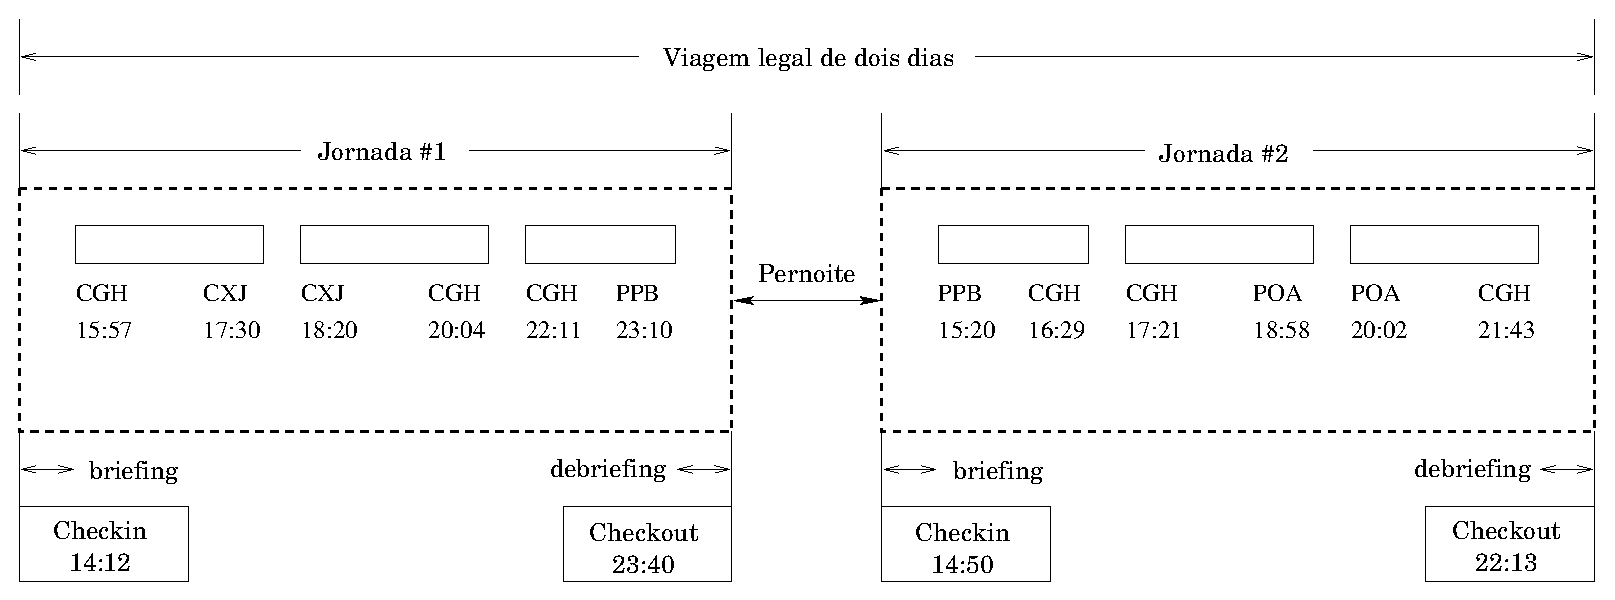
\includegraphics[width=0.98\linewidth]{pairing}
\end{center}
%
Implementamos e comparamos três métodos de solução do PDV: um algoritmo baseado em busca 
local, um algoritmo genético híbrido e um procedimento exato de geração de colunas para resolução
do PL relaxado.
}

%%%%%%%%%%%%%%%%%%%%%%%%%%%%%%%%%%%%%%%%%%%%%%%%%%%%%%%%%%%%%%%%%%%%%%%%%%%%%%
\headerbox{Formulação}{name=formulacao,column=0,below=introducao}{
%%%%%%%%%%%%%%%%%%%%%%%%%%%%%%%%%%%%%%%%%%%%%%%%%%%%%%%%%%%%%%%%%%%%%%%%%%%%%%
O PDV pode ser formulado como um problema de PLI conhecido por 
{\bf Set Cover}. Seja $c_j$ o custo da viagem $j$. Seja $x_j = 1$ se a viagem $j$ for escolhida 
($x_j = 0$ caso contrário). Seja $y_i \in \N$ o número de vezes que o voo $i$ é coberto com custo 
$d_i$ associado. Definindo $a_{ij} = 1$ se a viagem $j$ cobre o voo $i$ ($a_{ij} = 0$ caso 
contrário), então queremos resolver
%
\begin{eqnarray*}
	\text{minimizar} && \displaystyle \sum_{j=1}^n c_j x_j + \sum_{i=1}^m d_i y_i \\
	\text{sujeito à} && \displaystyle \sum_{j=1}^n a_{ij} x_j - y_i = 1 \ev \;\; i = 1, \ldots, m \\
	                 && x_j \in \{0, 1\} \ev \;\; j = 1, \ldots, n \\
	                 && y_i \geq 0 \ev \;\; i = 1, \ldots, m \ep
\end{eqnarray*}
%
Dado que o problema é NP-difícil e que existe um número enorme de variáveis (viagens possíveis), 
métodos heurísticos devem ser aplicados.
}


%%%%%%%%%%%%%%%%%%%%%%%%%%%%%%%%%%%%%%%%%%%%%%%%%%%%%%%%%%%%%%%%%%%%%%%%%%%%%%
\headerbox{Gerador de Viagens}{name=gerador,column=0,below=formulacao,above=bottom}{
%%%%%%%%%%%%%%%%%%%%%%%%%%%%%%%%%%%%%%%%%%%%%%%%%%%%%%%%%%%%%%%%%%%%%%%%%%%%%%
As viagens para otimização são geradas a partir de uma {\bf busca em profundidade} na rede de voos 
do problema. Os nós representam pontos de partida e chegada dos voos e arcos são adicionados toda 
vez que for possível estabelecer uma conexão legal entre os voos. Os voos que partem da base da 
tripulação são ligados à fonte $s$. Os voos que chegam na base são ligados ao sorvedouro $t$. Toda 
viagem viável representa um caminho $s-t$ no grafo.
%
\begin{center}
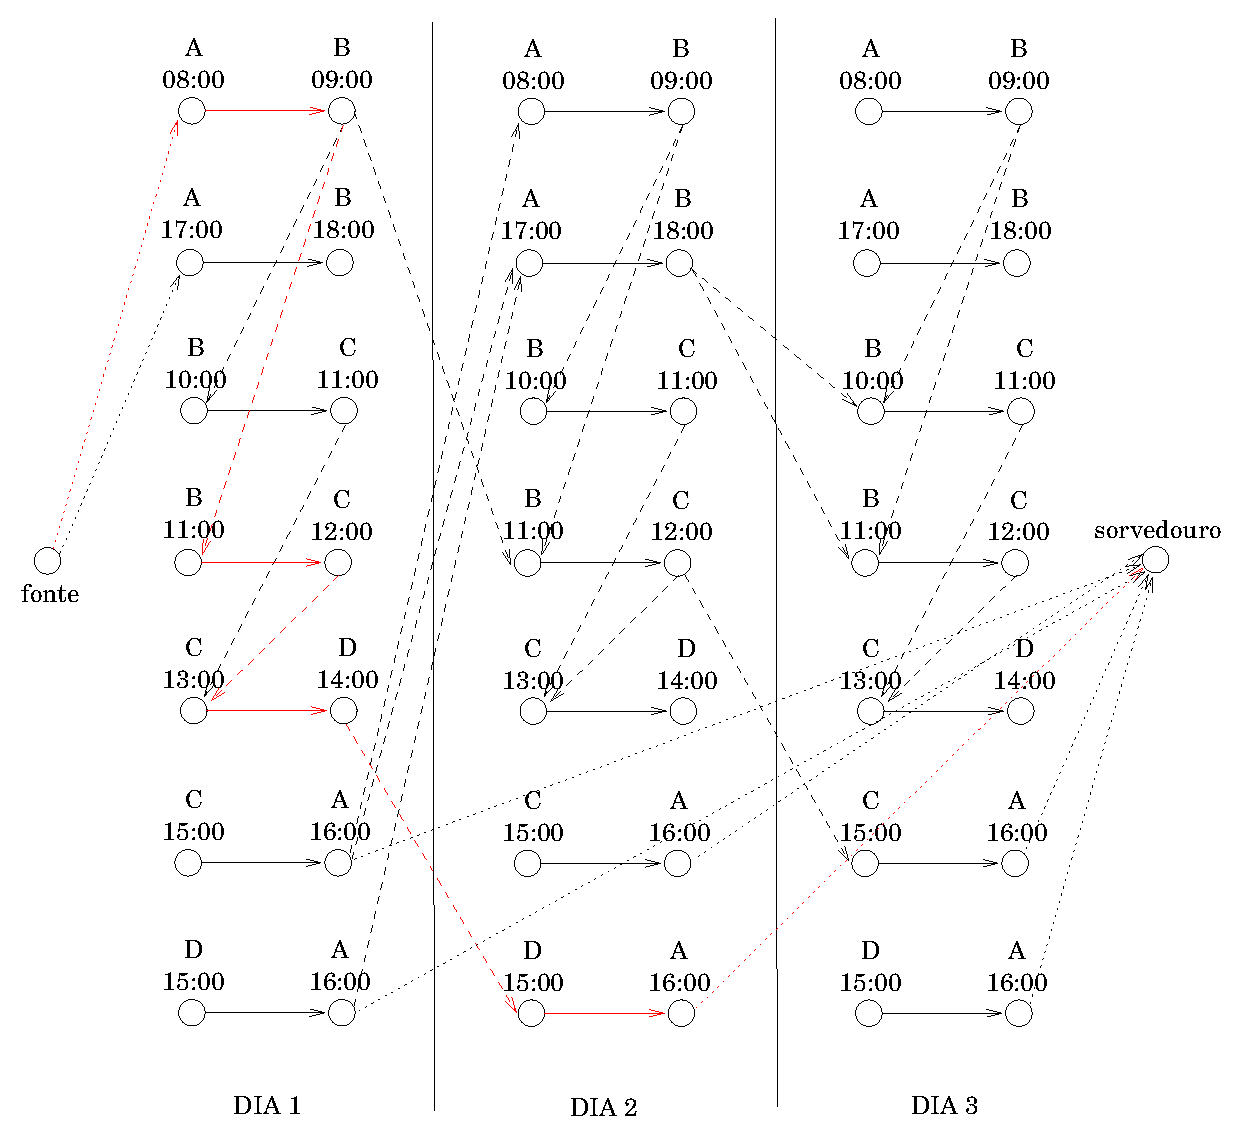
\includegraphics[width=0.98\linewidth]{network}
\end{center}
}


%%%%%%%%%%%%%%%%%%%%%%%%%%%%%%%%%%%%%%%%%%%%%%%%%%%%%%%%%%%%%%%%%%%%%%%%%%%%%%
\headerbox{Análise Preliminar}{name=preliminar,column=1,row=0}{
%%%%%%%%%%%%%%%%%%%%%%%%%%%%%%%%%%%%%%%%%%%%%%%%%%%%%%%%%%%%%%%%%%%%%%%%%%%%%%
Resolvemos de maneira exata o PDV para uma instância de voos da ponte aérea utilizando os 
otimizadores {\bf GLPK} e {\bf CPLEX}. 

Dado o número enorme de variáveis geradas, os problemas não puderam ser resolvidos em tempo 
aceitável (24 horas), mesmo para um número pequeno de pernas (voos).
%
\begin{center}
\includegraphics[width=0.92\linewidth]{preliminary}
\end{center}
}


%%%%%%%%%%%%%%%%%%%%%%%%%%%%%%%%%%%%%%%%%%%%%%%%%%%%%%%%%%%%%%%%%%%%%%%%%%%%%%%
\headerbox{Busca Local}{name=local,column=1,below=preliminar}{
%%%%%%%%%%%%%%%%%%%%%%%%%%%%%%%%%%%%%%%%%%%%%%%%%%%%%%%%%%%%%%%%%%%%%%%%%%%%%%%
\begin{center}
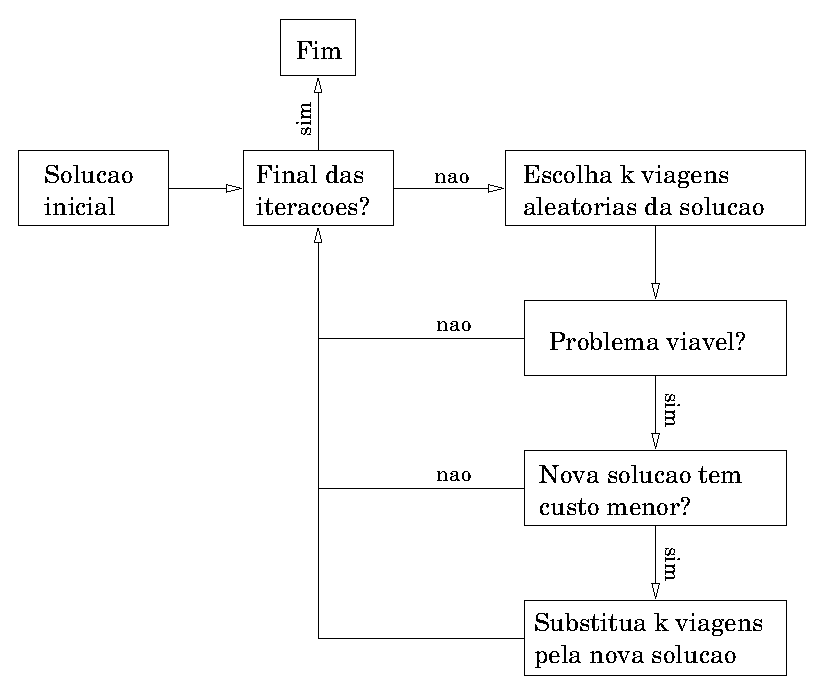
\includegraphics[width=0.85\linewidth]{local}
\end{center}
}


%%%%%%%%%%%%%%%%%%%%%%%%%%%%%%%%%%%%%%%%%%%%%%%%%%%%%%%%%%%%%%%%%%%%%%%%%%%%%%
\headerbox{Algoritmo Genético}{name=genetico,column=2,row=0}{
%%%%%%%%%%%%%%%%%%%%%%%%%%%%%%%%%%%%%%%%%%%%%%%%%%%%%%%%%%%%%%%%%%%%%%%%%%%%%%
\begin{center}
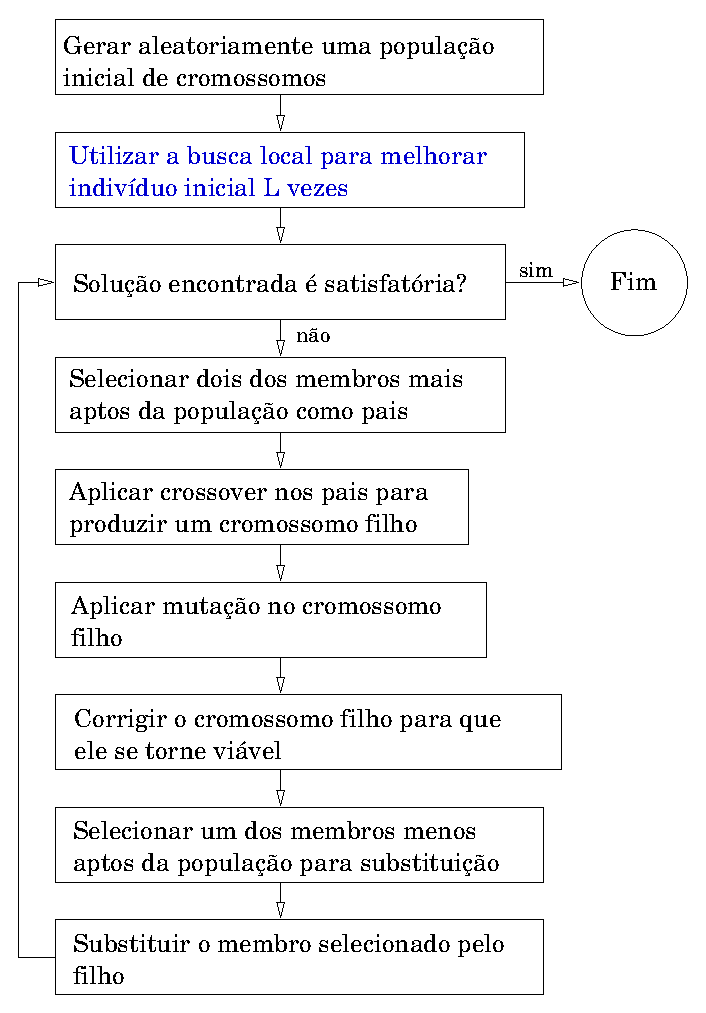
\includegraphics[width=0.835\linewidth]{genetic}
\end{center}
}


%%%%%%%%%%%%%%%%%%%%%%%%%%%%%%%%%%%%%%%%%%%%%%%%%%%%%%%%%%%%%%%%%%%%%%%%%%%%%%
\headerbox{Geração de Colunas}{name=cg,column=2,below=genetico}{
%%%%%%%%%%%%%%%%%%%%%%%%%%%%%%%%%%%%%%%%%%%%%%%%%%%%%%%%%%%%%%%%%%%%%%%%%%%%%%
\begin{center}
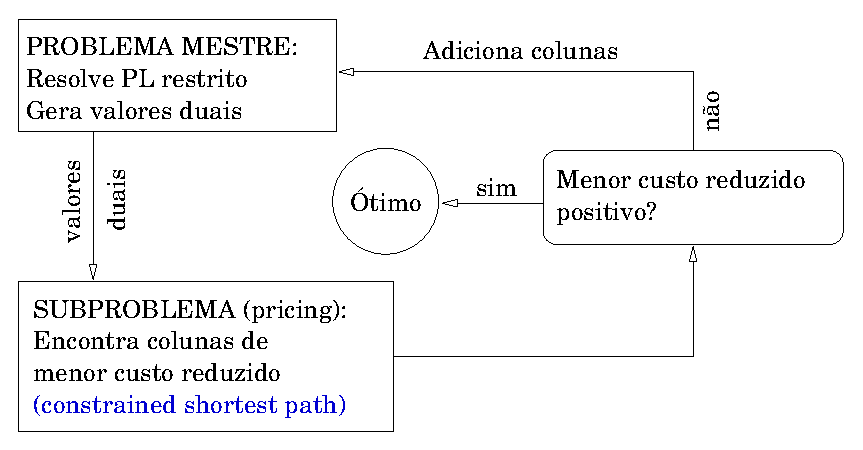
\includegraphics[width=0.85\linewidth]{cg}
\end{center}
}


%%%%%%%%%%%%%%%%%%%%%%%%%%%%%%%%%%%%%%%%%%%%%%%%%%%%%%%%%%%%%%%%%%%%%%%%%%%%%%
\headerbox{Conclusões}{name=conclusoes,column=1,above=bottom}{
%%%%%%%%%%%%%%%%%%%%%%%%%%%%%%%%%%%%%%%%%%%%%%%%%%%%%%%%%%%%%%%%%%%%%%%%%%%%%%
\begin{itemize}
\item A geração de colunas é rápida e fornece um limitante inferior para o custo da solução.
\item A busca local é eficiente e mostrou bons resultados em todas as instâncias para $k = 3$.
\item O algoritmo genético converge rapidamente para um mínimo local com $L$ suficientemente 
grande.
\end{itemize}
}

%%%%%%%%%%%%%%%%%%%%%%%%%%%%%%%%%%%%%%%%%%%%%%%%%%%%%%%%%%%%%%%%%%%%%%%%%%%%%%
\headerbox{Resultados}{name=resultados,column=1,span=2,below=cg,above=conclusoes}{
%%%%%%%%%%%%%%%%%%%%%%%%%%%%%%%%%%%%%%%%%%%%%%%%%%%%%%%%%%%%%%%%%%%%%%%%%%%%%%
\begin{center}
\includegraphics[width=0.95\linewidth]{results}
\end{center}
\begin{center}
\scalebox{0.81}{
\begin{tabular}{cc|c|c|c|c|c|c|c|c|c|c|}
	\cline{3-12}
	& &
	\multicolumn{2}{|c|}{\bf 26 voos} & 
	\multicolumn{2}{|c|}{\bf 48 voos} & 
	\multicolumn{2}{|c|}{\bf 92 voos} & 
	\multicolumn{2}{|c|}{\bf 340 voos} & 
	\multicolumn{2}{|c|}{\bf 62 voos PA} \\
	\cline{3-12}
	& & OBJ (DH) & CPU & OBJ (DH) & CPU & OBJ (DH) & CPU & OBJ (DH) & CPU & OBJ (DH) & CPU \\

	\hline
	\multicolumn{2}{|c|}{GC} & 
	5,696 (0)  & 0,26  & 
	6,230 (0) & 0,54  & 
	10,973 (0) & 1,36  & 
	42,744 (0) & 54,02 & 
	10,103 (0) & 1,13 \\

	\hline
	\multicolumn{1}{|c|}{\multirow{3}{*}{BL}} 
	& $k = 2$ & 
	0\% (0) & 1,10   & 
	>100\% (116) & 1,22   & 
  >100\% (124) & 3,16   & 
	>100\% (654) & 208,44 & 
	>100\% (8) & 0,79 \\
	\multicolumn{1}{|c|}{} 
	& $k = 3$ &
	0\% (0) & 1,48    & 
	14,1\% (0) & 7,91    & 
	8,1\% (0) & 18,68   & 
	32,5\% (9) & 1303,53 & 
	87,7\% (0) & 1,31 \\
	\multicolumn{1}{|c|}{} 
	& $k = 4$ & 
	0\% (0) & 1,81 & 
	0\% (0) & 11,46 & 
	7,7\% (0) & 99,09 & 
	25,5\% (11) & 2182,31 & 
	0\% (0)   & 17,83 \\

	\hline
	\multicolumn{1}{|c|}{\multirow{3}{*}{AG}} 
	& $L = 1$ & 
	0\% (0) & 1,39 & 
	78,1\% (2) & 4,35 & 
	>100\% (9) & 8,30 & 
	>100\% (476) & 1074,97 & 
	56,2\% (0) & 4,31 \\
	\multicolumn{1}{|c|}{} 
	& $L = 5$ & 
	0\% (0) & 4,17 & 
	13,8\% (0) & 13,19 & 
	46,4\% (0) & 10,79 & 
	>100\% (208) & 763,19 & 
	36,2\% (0) & 13,99 \\
	\multicolumn{1}{|c|}{} 
	& $L = 10$ & 
	0\% (0) & 11,01 & 
	0\% (0) & 33,99 & 
	72,2\% (3) & 17,85 & 
	>100\% (78) & 482,10 & 
	30,5\% (0) & 27,50 \\
	\hline
\end{tabular}
}
\end{center}
\vspace{-0.25cm}
\begin{smaller}
GC = geração de colunas. BL = busca local. AG = algoritmo genético. PA = ponte aérea.
OBJ = valor da função objetivo (\% indica a diferença em relação à GC). DH = número de voos 
sobrecobertos ({\it deadheadings}). CPU = tempo de processamento em segundos. $k$ = número de 
viagens sorteadas na BL. $L$ = número de otimizações no indivíduo inicial no AG. 
\end{smaller}
}

%%%%%%%%%%%%%%%%%%%%%%%%%%%%%%%%%%%%%%%%%%%%%%%%%%%%%%%%%%%%%%%%%%%%%%%%%%%%%%
\headerbox{Perspectivas}{name=perspectivas,column=2,above=bottom,below=resultados}{
%%%%%%%%%%%%%%%%%%%%%%%%%%%%%%%%%%%%%%%%%%%%%%%%%%%%%%%%%%%%%%%%%%%%%%%%%%%%%%
\begin{itemize}
\item Implementação de um esquema branch-and-price para obtenção de solução inteira a parir da 
geração de colunas.
\item Combinação e paralelização das heurísticas estudadas, explorando os pontos fortes de cada uma 
delas.
\item Possível sistema comercial.
\end{itemize}
}

\end{poster}
\end{document}
